\newpage
\chapter {Prototipo Realizzato}

Di seguito verrà fornita una descrizione delle componenti principali che costituiscono il prototipo realizzato, e in particolare verrà descritto come le soluzioni progettate sono state realizzate nella pratica. Dove necessario, verranno riportati listati di codice sorgente a supporto della descrizione.

\section{Simulazione}

	\begin{figure}[htbp]
		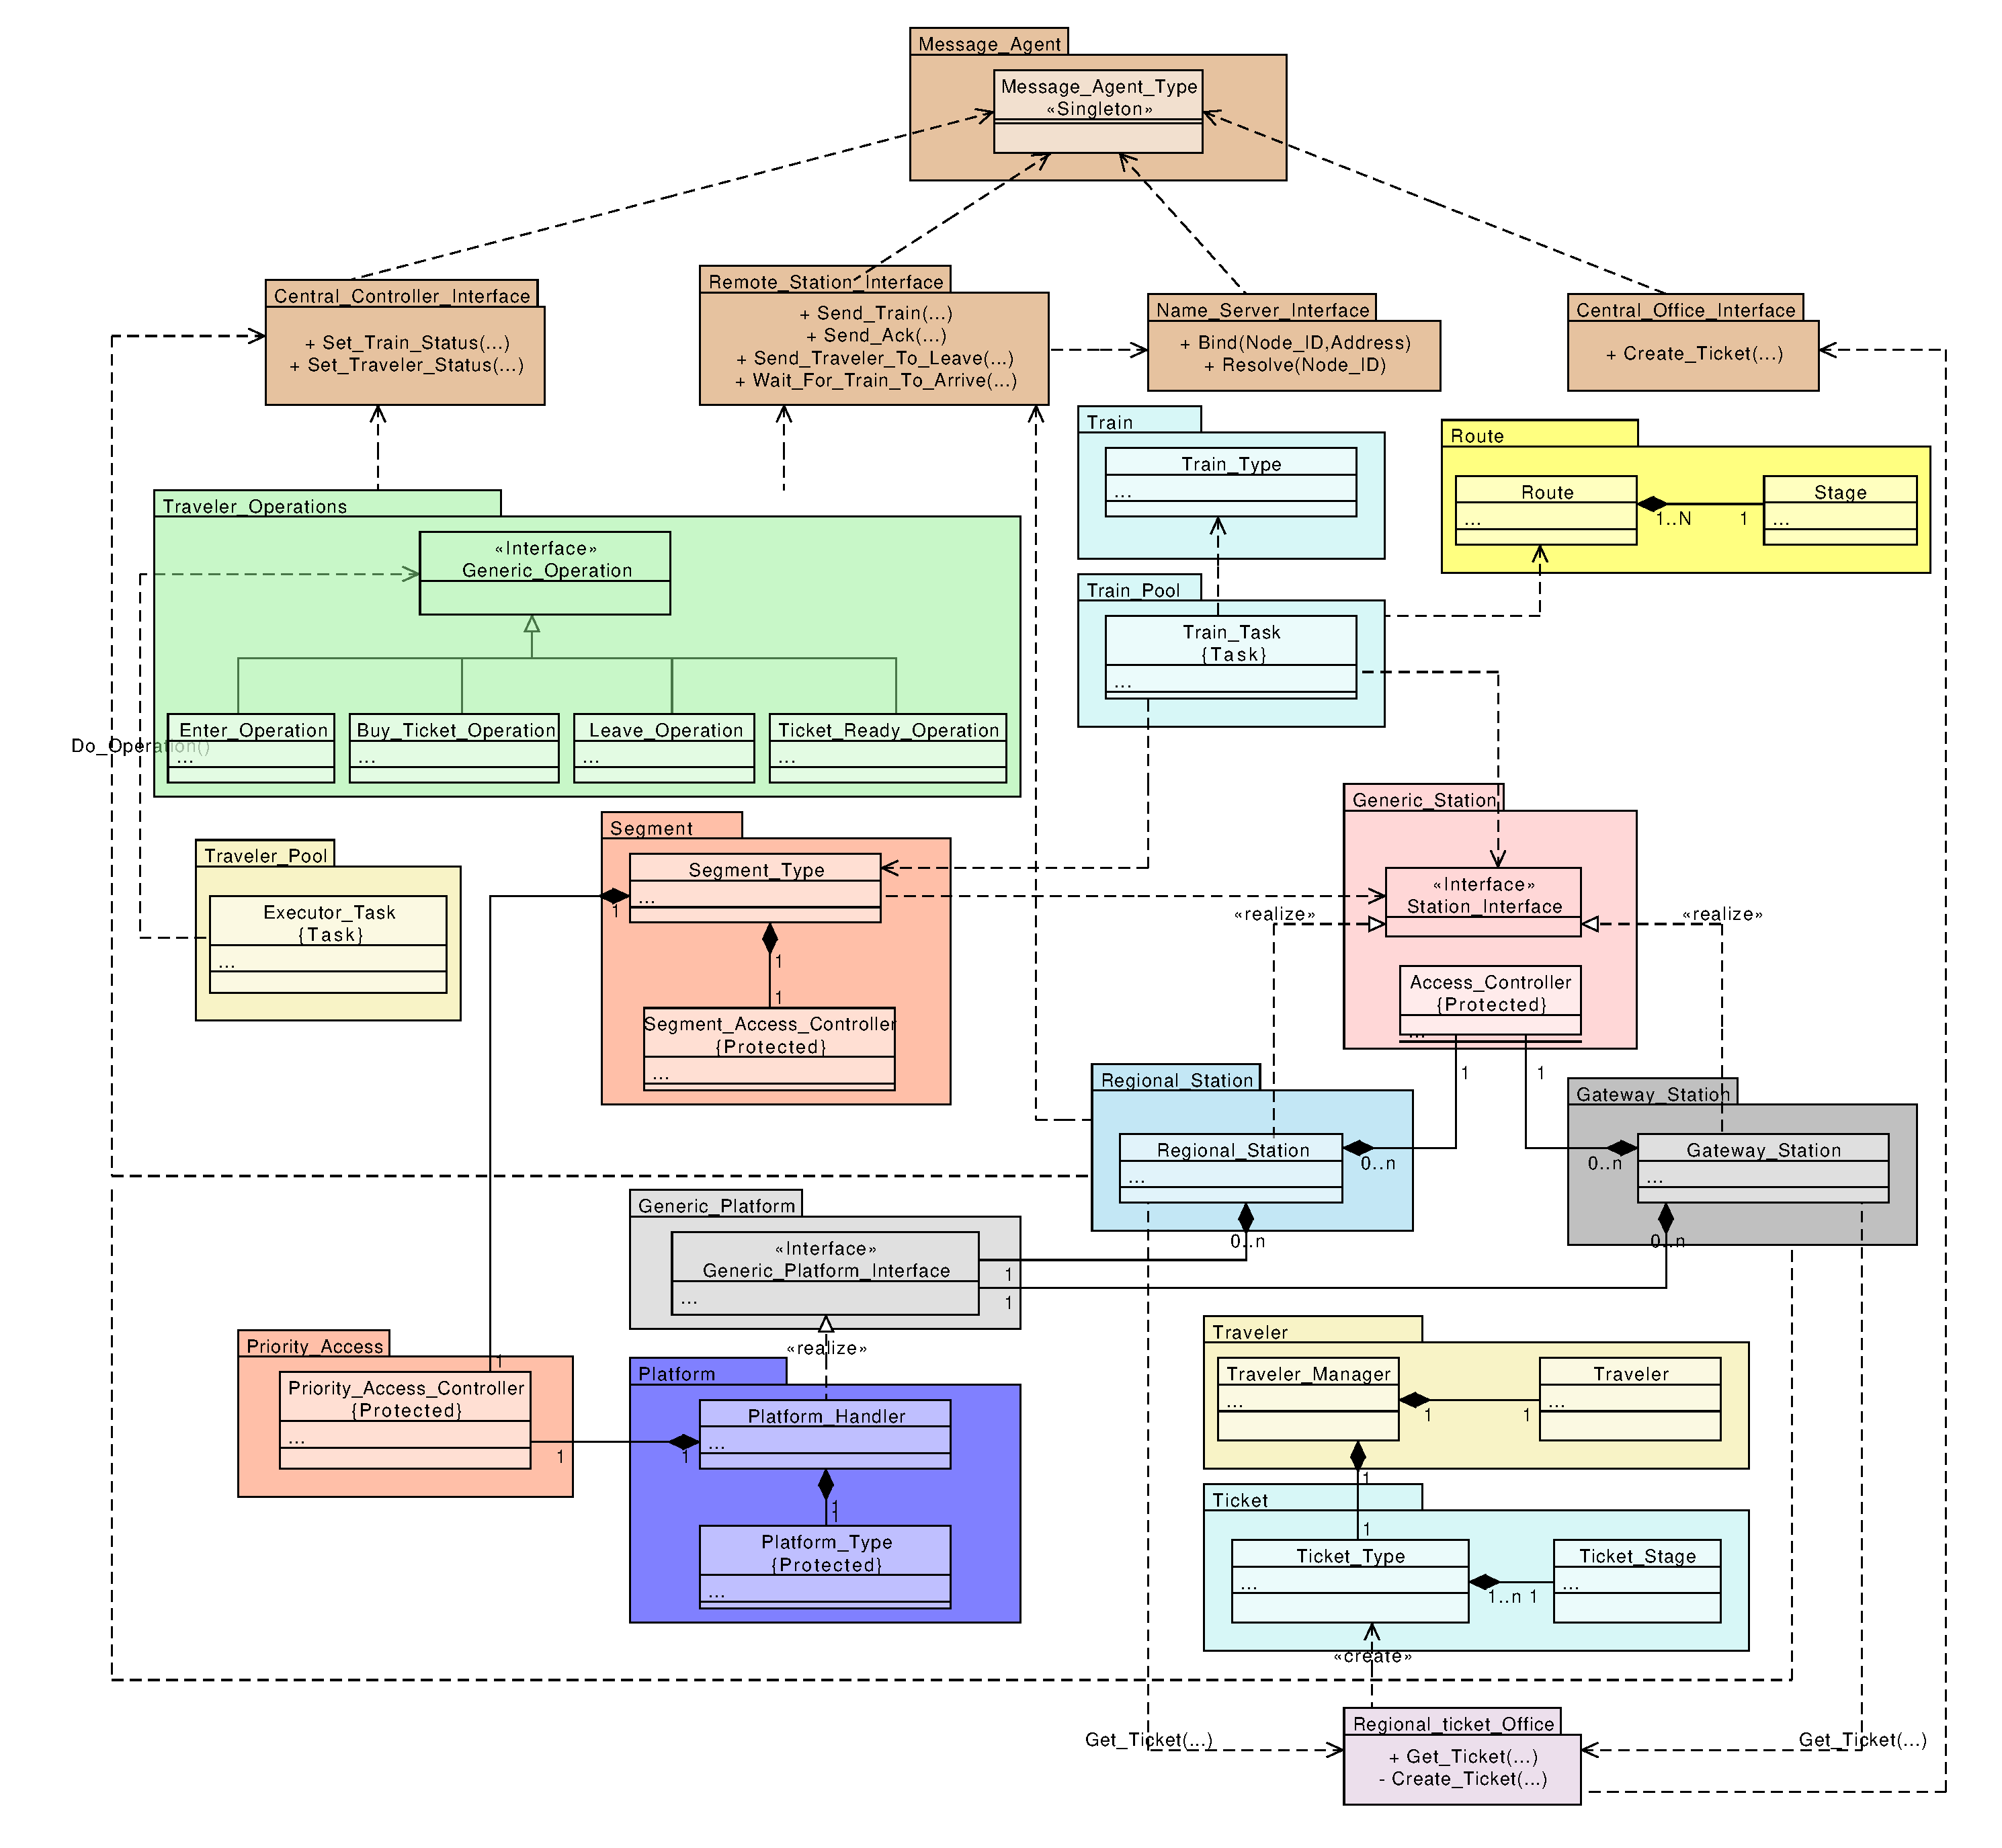
\includegraphics[scale=0.40,trim= 90mm 0mm 0mm 0mm]{imgs/Simplified_Class_Diagram.pdf}
		\caption{\footnotesize{Diagramma delle classi che illustra le componenti e le relazioni più significative che coinvolgono la simulazione.}}
		\label{img:class_diagram}
	\end{figure}

L'architettura di massima adottata per la realizzazione del core di simulazione, è visibile nel diagramma delle classi in figura \ref{img:class_diagram} nel quale, per brevità, sono stati riportati solo le informazioni più significative, omettendo per esempio i package nei quali sono contenute gli oggetti creati duarante l'esecuzione.
	
	Viene ora fornita una breve descrizione delle varie componenti che sono state utilizzate, procedendo per Package. Nelle sezioni seguenti si utilizzeranno le nozioni di \ii{Task} e \ii{Tipo protetto} definite dal linguaggio \ii{Ada}, utilizzato per l'implementazione, e verrà mostrato come le soluzioni presentate nel capitolo \ref{chapter:solution} sono state tradotte con strumenti di linguaggio.

	\subsection{Message\_Agent}
	
	Il package \ttt{Message\_Agent} fornisce un'interfaccia per l'invio di messaggi remoti. Esso contiene una classe singleton \ttt{Message\_Agent\_Type}, la quale possiede i seguenti campi dato:
	\begin{description}
		\item \ttt{- Client\_Agent : YAMI.Agents.Agent\_Access} \\
		Campo dati privato di tipo \ttt{YAMI.Agents.Agent\_Access} che contiene una istanza di Agente fornito dalla libreria \ii{Yami4}, e che viene utilizzato per l'invio e la ricezione di messaggi remoti.
		\item \ttt{- Handlers\_Map : Map} \\
		Hash-map privata, la quale associa a chiavi di tipo \ttt{String}, valori di tipo \ii{riferimento a procedura}; essa viene utilizzata per associare a ciascun servizio offerto dall'oggetto \ttt{Client\_Agent} un handler per la sua gestione.
	\end{description}
	
	Essa offre inoltre i seguenti metodi:
	
	\begin{description}
		\item \ttt{+ Listen\_To(Server\_Address)} \\
		Indica all'oggetto \ttt{Client\_Agent} di rimanere in ascolto presso l'indirizzo \ttt{Server\_Address}, attraverso il quale riceverà tutti i messaggi destinati al nodo. Nella fase di registrazione dell'oggetto remoto, viene definito un handler per la ricezione dei messaggi, il quale effettua il dispatching di ciascun messaggio ricevuto invocando la procedura corrispondente al servizio richiesto, definita nella mappa \ttt{Handlers\_Map}.
		
		\item \ttt{+ Close()} \\
		Chiude la connessione dell'oggetto \ttt{Client\_Agent}.
		
		\item \ttt{+ Send\_Message(\\
			Destination\_Address:String,\\
			Object:String,\\
			Service:String,\\
			Params:YAMI.Parameters.Parameters\_Collection,\\
			Callback)}\\
		Invia un messaggio all'oggetto remoto indicato da \ttt{Object} all'indirizzo \ttt{Destination\_Address}, richiedendo il servizio \ttt{Service}, e con i parametri indicati da \ttt{Params}. Se non nulla, la funzione di callback \ttt{Callback} viene invocata alla ricezione del messaggio di risposta, altrimenti quest'ultimo viene ignorato.
		
		\item \ttt{+ Send\_One\_Way(\\
			Destination\_Address : String,\\
			Object 				: String,\\
			Service 			: String,\\
			Params 				: YAMI.Parameters.Parameters\_Collection)}\\
		Metodo simile a \ttt{Send\_Message}, solo che non rimane in attesa della risposta al messaggio inviato.
	\end{description}
	
	Nessun meccanismo di serializzazione delle richieste è stato adottato, in quanto esso è già operato dagli oggetti della libreria \ii{Yami4}.
	
	\subsection{Central\_Controller\_Interface}
	
	Il package \ttt{Central\_Controller\_Interface} fornisce un'interfaccia per permettere alle entità della simulazione di inviare un evento di notifica all'oggetto remoto \ttt{central\_controller}. A tal proposito sono messi a disposizione le procedure \ttt{Set\_Train\_Status} e \ttt{Set\_Traveler\_Status}, le quali effettuano il marshalling dei dati in ingresso (in formato \ttt{JSON}) e inviano un messaggio remoto mediante il metodo \ttt{Send\_One\_Way} offerto dall'unica istanza di \ttt{Message\_Agent\_Type}.
	
	\subsection{Central\_Office\_Interface}
	
	Il package \ttt{Central\_Office\_Interface} fornisce un'interfaccia per permettere la comunicazione con la Biglietteria Centrale, mediante l'invio di messaggi all'oggetto remoto \ttt{central\_ticket\_server}.
	
		\begin{description}
			\item \ttt{+ Create\_Ticket( \\
				From : String,\\
				To	 : String,\\
				Traveler\_Index: Integer)} \\
			Richiede la creazione di un Biglietto inviando un messaggio remoto mediante il metodo \ttt{Send\_Message} offerto dall'unica istanza di \ttt{Message\_Agent\_Type}. Non viene specificata una procedura di callback, in quanto il risultato verrà inviato dalla Biglietteria Centrale una volta calcolato il Biglietto.
			
			\item \ttt{+ Validate(\\
				The\_Ticket:Ticket,\\
				Callback:access procedure(The\_Ticket:Ticket,Response:Boolean))}\\
			Richiede la validazione di un Biglietto inviando un messaggio remoto mediante il metodo \ttt{Send\_Message} offerto dall'unica istanza di \ttt{Message\_Agent\_Type}. La richiesta è sincrona, e la risposta viene quindi elaborata e viene invocata la procedura \ttt{Callback} passando come parametri i risultati estratti.
			
			\item \ttt{+ Update\_Run(\\
				Route\_Index:Integer,\\
				Current\_Run:Integer,\\
				Callback:access procedure(...))}\\ 
			Invia un messaggio remoto per comunicare l'aggiornamento della corsa corrente \ttt{Current\_Run} per il percorso \ttt{Route\_Index}. Nel caso in cui la corsa sia l'ultima delle $N$ mantenute, viene creata una nuova Time Table per il percorso \ttt{Route\_Index} dalla Biglietteria Centrale che viene restituito al chiamante. Nel caso in cui essa venga ricevuta (in formato \ttt{JSON}), viene effettuato l'unmarshalling e creata l'istanza corrispondente di \ttt{Time\_Table\_Type} da sostituire a quella corrente.
			
			\item \ttt{+ Load\_Time\_Tables(\\
				Callback:access procedure(Table:Time\_Table\_Array\_Ref))}\\
			Invocazione di un messaggio remoto per richiedere l'insieme delle Time Tables per tutti i percorsi.
				
		\end{description}
	
	\subsection{Name\_Server\_Interface}
	
	Package che fornisce un'interfaccia remota per la comunicazione con il Server dei Nomi che mantiene la lista delle Regioni di simulazione. Esso fornisce le seguenti procedure:
	\begin{description}
		\item \ttt{+  Bind(\\
		Name\_Server : String,\\
		Node\_Name 	: String,\\
		Address	: String)} \\
		
	Permette di registrare presso il Server dei Nomi che l'entità remota \ttt{Node\_Name} è disponibile alla locazione indicata da \ttt{Address}. 
	
	\item \ttt{+  Resolve(\\
		Name\_Server : String,\\
		Node\_Name 	: String),\\
		Callback : access procedure(Result:String)} \\
		
		Permette di richiedere al Server dei Nomi la risoluzione della locazione alla quale si trova l'entità \ttt{Node\_Name}. Una volta che la risposta è disponibile, viene invocata la procedura di callback \ttt{Callback}. 
				
	\end{description}
	
	Per entrambe le procedure, viene inviato un messaggio all'oggetto remoto identificato da \ttt{name\_server}, mediante il metodo \ttt{Send\_Message} di \ttt{Message\_Agent\_Type}, al quale viene passato una procedura di callback che estrae il campo \ttt{address} dal messaggio di ritorno e lo passa all'invocazione di \ttt{Callback}. Presso il package viene mantenuta una hash-map, la quale permette di memorizzare le destinazioni risolte, in modo da limitare l'invio di messaggi remoti.
	
	\subsection{Remote\_Station\_Interface}
	
	Il package \ttt{Remote\_Station\_Interface} espone un insieme di procedure che permettono l'invio di messaggi remoti tra i Nodi che cooperano alla simulazione, che saranno diretti agli oggetti remoti \ttt{message\_handler}.
	\begin{description}
		
		\item \ttt{+ Send\_Train(\\
			Train\_Descriptor\_Index:Integer,\\
			Station:Integer,\\
			Platform:Integer,\\
			Next\_Node\_Name:String)}\\ 
		Tale procedura permette l'invio di un messaggio remoto al Nodo identificato da \ttt{Next\_Node\_Name} per effettuare il trasferimento del Treno indicato da \ttt{Train\_Descriptor\_Index} presso la Stazione \ttt{Station}, Piattaforma \ttt{Platform}. 
		
		\item \ttt{+ Train\_Left\_Message(\\
			Train\_Descriptor\_Index:Integer,\\
			Station:Integer,\\
			Platform:Integer,\\
			Next\_Node\_Name:String)}\\ 
		Questa procedura permette l'invio di un messaggio remoto al Nodo identificato da \ttt{Next\_Node\_Name} per indicare la partenza del Treno \ttt{Train\_Descriptor\_Index} dalla Piattaforma \ttt{Platform} della Stazione \ttt{Station}.
		
		\item \ttt{+ Send\_Traveler\_To\_Leave(\\
			Traveler\_Index:Integer,\\
			Train\_ID:Integer,\\
			Station:Integer,\\
			Platform:Integer,\\
			Node\_Name:String)}\\
		Permette l'invio di un messaggio remoto al Nodo identificato da \ttt{Node\_Name} per aggiungere il Viaggiatore \ttt{Traveler\_Index} in attesa presso la Piattaforma \ttt{Platform} della Stazione \ttt{Station} dell'arrivo del Treno \ttt{Train\_ID} per poter lasciare tale Stazione.
		
		\item \ttt{+ Wait\_For\_Train\_To\_Arrive(\\
			Next\_Station:Integer,\\
			Traveler\_Manager\_Index:Integer,\\
			Train\_ID:Integer,\\
			Destination\_Platform\_Index:Integer,\\
			Next\_Region:String)}\\
		Permette l'invio di un messaggio remoto al Nodo identificato da \ttt{Node\_Name} per aggiungere il Viaggiatore \ttt{Traveler\_Index} in attesa presso la Piattaforma \ttt{Platform} della Stazione \ttt{Station} dell'arrivo del Treno \ttt{Train\_ID} per poter arrivare presso tale Stazione.
		
	\end{description}
	
	\subsection{Queue}
	
	Il package \ttt{Queue} contiene la definizione di alcuni tipi di code utilizzati nell'intera simulazione:
		\begin{description}
			\item {\ttt{Terminable\_Queue}} \\
			Tipo \ii{protetto} costruito come \ii{wrapper} della coda standard offerta dal package \ttt{Ada.Containers.Unbounded\_Synchronized\_Queues}, e che permette di interrompere l'attesa sulla guardia Booleana definita per l'entry \ttt{Dequeue}, la quale rimane chiusa nel caso in cui non vi siano più elementi al suo interno.
			Esso e definisce l'entry
			\begin{center}
				\ttt{Dequeue(Element:out  Element\_Type,Terminated:out  Boolean)}
			\end{center}
		
		con guardia Booleana: \ttt{Termination or Q.Current\_Use > 0}, dove \ttt{Q} è una coda fornita dalle librerie standard di linguaggio, \ttt{Current\_Use} è una funzione che restituisce il numero di elementi all'interno della coda, e \ttt{Termination} è un campo dati Booleano della risorsa protetta. In questo modo nel caso in cui il valore di \ttt{Termination} sia \ttt{True} l'attesa su coda viene interrotta, e viene restituito al chiamante il valore \ttt{True} attraverso il parametro passato per riferimento \ttt{Terminated}, altrimenti la coda restituisce anche il valore del primo elemento rimosso dalla coda.
		
		Per poter attribuire al campo dati \ttt{Termination} il valore \ttt{True}, viene fornita la procedura protetta \ttt{Stop}.
			
			\item {\ttt{Limited\_Simple\_Queue}} \\
			Tipo di coda non thread-safe, di dimensione limitata, realizzato mediante un array di elementi, e che fornisce un'interfaccia composta dai metodi:
			\begin{itemize}
				\item \ttt{Enqueue(Element:Element\_Type)} per accodare un nuovo elemento;
				\item \ttt{Dequeue(Element:out Element\_Type)} per rimuovere l'elemento dalla testa della coda;
				\item \ttt{Get(Index:Integer)} per ottenere il valore dell'elemento nella posizione \ttt{Index};
			\end{itemize}
			
			\item {\ttt{Unlimited\_Simple\_Queue}} \\
			Tipo di coda non thread-safe di dimensione illimitata, realizzato mediante un oggetto di tipo \ttt{Vector} definito dalle librerie standard \ttt{Ada.Containers.Vectors}. Esso presenta un'interfaccia del tutto simile a quella offerta dal tipo \ttt{Limited\_Simple\_Queue}, alla quale aggiunge il metodo \ttt{Is\_Empty : Boolean} che indica se la coda è vuota. 
			
		\end{description}
	
	\subsection{Generic\_Operation\_Interface}
	
	Package che contiene la definizione di una interfaccia \ttt{Operation\_Interface}, la quale espone un unico metodo \ttt{Do\_Operation()}. Essa rappresenta una generica operazione. Viene definito inoltre un tipo puntatore ad operazione generica \ttt{Any\_Operation}.
	
	\subsection{Traveler\_Pool}
	
	Il package {Traveler\_Pool} realizza il meccanismo per l'esecuzione delle entità Viaggiatore descritto in sezione \ref{subsec:traveler_def}. Esso mantiene 
	\begin{itemize}
		\item una coda \ttt{Operations\_Queue} di puntatori di tipo \ttt{Any\_Operation} a operazioni. Tale coda è di tipo \ttt{Terminable\_Queue}, definito nel package \ttt{Queue}.
		\item la definizione di un tipo record \ttt{Traveler\_Pool\_Type} contenente un array di oggetti task \ttt{Executor}, di dimensione fissata in fase di creazione.
		Ciascun task di tipo \ttt{Executor} eseguirà semplici operazioni ciclicamente:
		\begin{itemize}
			\item Estrae il primo elemento dalla coda \ttt{Operations\_Queue} mediante il metodo \ttt{Dequeue} da essa offerto. 
			\item Nel caso in cui il valore del parametro \ttt{Terminated} passato per riferimento abbia il valore \ttt{True}, allora viene interrotto il ciclo di operazioni.
			\item Altrimenti, viene invocato il metodo \ttt{Do\_Operation} sul puntatore ad operazione estratto.
		\end{itemize}
	\end{itemize}
	
	\subsection{Ticket}
	
	Package che contiene la definizione di un Biglietto. Esso definisce infatti il tipo record \ttt{Ticket\_Type}, il quale è composto da un campo intero \ttt{Next\_Stage} che indica la tappa corrente del percorso descritto dal Biglietto, e un puntatore ad un array di Tappe, ovvero di oggetti di tipo \ttt{Ticket\_Stage}. Quest'ultimi mantengono le seguenti informazioni:
		\begin{itemize}
			\item \ttt{Start\_Station} : Indice della Stazione di partenza;
			\item \ttt{Next\_Station} : Indice della prossima Stazione;
			\item \ttt{Train\_ID} : Identificativo del Treno da utilizzare per raggiungere la stazione \ttt{Next\_Station};
			\item \ttt{Start\_Platform\_Index} : Indice della Piattaforma di partenza;
			\item \ttt{Destination\_Platform\_Index} : Indice della Piattaforma di destinazione;
			\item \ttt{Region} : Nome della regione nella quale si colloca la stazione \ttt{Next\_Station};
		\end{itemize}
	Il package fornisce inoltre le funzioni necessarie per effettuare marshalling e unmarshalling degli oggetti di tipo \ttt{Ticket\_Type} in/dal formato \ttt{JSON}.
	
	\subsection{Traveler}
	
	Package che contiene la definizione del tipo rappresentante un Viaggiatore. In esso infatti viene definito il tipo record \ttt{Traveler\_Manager}, formato dai campi:
		\begin{itemize}
			\item \ttt{Next\_Operation} : Indice della prossima operazione da eseguire;
			\item \ttt{Destination} : Nome della stazione di destinazione;
			\item \ttt{Start\_Station} : Nome della stazione di partenza;
			\item \ttt{Start\_Region} : Regione di partenza;
			\item \ttt{Traveler} : Campo di tipo record che contiene alcuni dati relativi al Viaggiatore, come nome e cognome.
			\item \ttt{Ticket} : Riferimento ad un oggetto di tipo \ttt{Ticket\_Type}.
		\end{itemize}
	Il package \ttt{Traveler} contiene inoltre le funzioni necessarie per effettuare marshalling e unmarshalling secondo il formato \ii{JSON}.
	
	
	\subsection{Regional\_Ticket\_Office}
	
	Il package \ttt{Regional\_Ticket\_Office} mantiene una tabella \ttt{Paths}, la quale per ciascuna Stazione della Regione corrente, definisce i percorsi più brevi per raggiungere ciascuna altra destinazione nella Regione. Esso inoltre espone la seguente interfaccia:
	\begin{description}
		\item \ttt{+ Create\_Ticket(From:String,To:String) : Ticket\_Type} \\
	Crea un istanza di oggetto \ttt{Ticket\_Type} che rappresenta un biglietto per raggiungere la destinazione \ttt{To} a partire da \ttt{From} nella regione corrente. Essa realizza l'algoritmo di creazione di un Biglietto descritto in sezione \ref{subsubsec:ticket_creation}.
		\item \ttt{+ Get\_Ticket (Traveler\_Index:Integer,From:String,To:String)} \\
	La procedure si occupa dell'effettiva creazione del Biglietto (oggetto di tipo \ttt{Ticket\_Type}). Tale procedura effettua un controllo: se le Stazioni \ttt{From} e \ttt{To} sono contenute all'interno della Regione corrente, allora procede alla creazione del Biglietto vero e proprio attraverso la funzione \ttt{Create\_Ticket}, che viene quindi assegnato al Viaggiatore di indice \ttt{Traveler\_Index}; successivamente viene inserita l'operazione \ttt{TICKET\_READY} nella coda di operazioni di \ttt{Traveler\_Pool}. Se invece la Stazione di destinazione \ttt{To} non è contenuta nella Regione corrente, allora viene richiesta la creazione del Biglietto alla Biglietteria Centrale attraverso l'interfaccia \ttt{Central\_Office\_Interface}.
	\end{description}
	
	Il package \ttt{Regional\_Ticket\_Office} contiene inoltre la procedura \ttt{Init\_Path\_Map} utilizzata per caricare la mappa contenente i percorsi più brevi, usata dall'algoritmo di creazione del Biglietto. 
	
		\subsection{Route}
	
	Il package \ttt{Route} contiene la definizione del tipo \ttt{Route\_Type}, array di oggetti di tipo \ttt{Stage}. Quest'ultimo è un tipo \ii{record} che si compone dei seguenti campi dato:
	\begin{itemize}
		\item \ttt{Start\_Station}: Indice della Stazione di partenza.
		\item \ttt{Next\_Station}: Indice della Prossima Stazione.
		\item \ttt{Start\_Platform}: Indice della Piattaforma di partenza.
		\item \ttt{Platform\_Index}: Indice della prossima Piattaforma.
        \item \ttt{Node\_Name}: Identificativo del Nodo sul quale si trova la prossima Stazione.
        \item \ttt{Next\_Segment}: Indice del prossimo Segmento da percorrere.
		\item \ttt{Leave\_Action}: Azione da intraprendere alla partenza dalla Stazione.
		\item \ttt{Enter\_Action}: Azione da intraprendere all'ingresso alla prossima Stazione.
	\end{itemize}
	
	Esso fornisce inoltre le procedure necessarie alla conversione da \ii{JSON} a oggetto \ttt{Route\_Type} e viceversa. Tutti gli oggetti Route sono mantenuti in un array nel package \ttt{Routes}.

	
		\subsection{Time\_Table}
	
	Il package \ttt{Time\_Table} contiene la definizione del tipo \ttt{Time\_Table\_Type}, che rappresenta una tabella di orari per una specifica \ttt{Route}. Esso è un \ii{record} con i seguenti campi:
	\begin{itemize}
		\item \ttt{Route\_Index}: Indice del Percorso per il quale la Tabella è definita.
		\item \ttt{Table}: Matrice di $NxM$ oggetti di tipo \ttt{Ada.Calendar.Time}, dove $N$ è il numero di Corse mantenute, e $M$ è la lunghezza della \ttt{Route} per la quale la tabella è definita.
		\item \ttt{Current\_Run}: Indice della Corsa corrente (da $1$ a $N$).
		\item \ttt{Current\_Run\_Cursor}: Indice utilizzato per scorrere gli orari memorizzati nella Corsa \ttt{Current\_Run}.
		\item \ttt{Current\_Run\_Id}: Identificativo univoco della Corsa. 
	\end{itemize}
	
	Il package oltre a definire le funzioni necessarie per effettuare la conversione da \ttt{JSON} a \ttt{Time\_Table\_Type} e viceversa, definisce la procedura 
\begin{lstlisting}
	Update_Time_Table(Table:access Time_Table_Type)} 
\end{lstlisting}
 la quale aggiorna il valore di \ttt{Current\_Run\_Cursor}. Nel caso in cui la corsa corrente \ttt{Current\_Run} sia esaurita (\ttt{Current\_Run\_Cursor + 1 > }$M$) allora \ttt{Current\_Run} viene incrementato e viene comunicato ciò alla Biglietteria Centrale mediante la procedura \ttt{Update\_Run} di \ttt{Central\_Office\_Interface}, la quale effettua una richiesta sincrona.
	L'insieme di tutte le tabelle è mantenuto in un array nel package \ttt{Environment}.

	
	\subsection{Train}
	
	Il package \ttt{Train} contiene la definizione del tipo \ttt{Train\_Descriptor}, record contenente tutti i dati che caratterizzano una entità Treno, e alcune funzioni necessarie ad effettuare la conversione da JSON a oggetto \ttt{Train\_Descriptor} e viceversa.
	I campi principali del record \ttt{Train\_Descriptor} sono:
	\begin{itemize}
		\item \ttt{Id}: identificativo univoco del Treno.
		\item \ttt{Speed}: Velocità di percorrenza Corrente.
	    \item \ttt{Max\_Speed}: Velocità massima raggiungibile dal Treno.
	    \item \ttt{Current\_Station} Indice della stazione corrente.
	    \item \ttt{Route\_Index}: Indice del Percorso assegnato al Treno.
	    \item \ttt{Next\_Stage}: Prossima tappa del Percorso assegnato.
	    \item \ttt{Sits\_Number}: Numero di posti a sedere.
	    \item \ttt{Occupied\_Sits}: Numero di posti occupati correntemente.
		\item \ttt{T\_Type}: Indica il tipo di Treno, tra \ttt{FB} e \ttt{REGIONAL}.
		\item \ttt{Start\_Node}: Regione dalla quale il Treno parte.
	\end{itemize}
	
	Tali descrittori sono memorizzati in un array \ttt{Trains} presso il package \ttt{Trains}, in modo tale da poter essere acceduti in modo diretto dalle varie componenti del sistema.
	
	\subsection{Train\_Pool}
	
	Il package \ttt{Train\_Pool} definisce il pool di Task, che serve ad eseguire le operazioni previste per i Treni. Esso mantiene due code (di tipo \ttt{Terminable\_Queue}) di valori interi, una per ciascuna categoria di Treno, nelle quali verranno inseriti gli indici dell'array di descrittori \ttt{Trains.Trains}, e definisce il tipo Task \ttt{Train\_Executor\_Task}, il quale effettua le seguenti operazioni ciclicamente:
	\begin{itemize}
		\item Preleva da una delle due code il prossimo indice dell'array di descrittori. 

\begin{lstlisting}
...
Trains.Queue.Dequeue(
	To_Get      => Current_Descriptor_Index,
	Terminated  => Terminated);
...
\end{lstlisting}

		\item Effettua la partenza dalla stazione corrente all'orario previsto dalla Time Table per il percorso assegnato al Treno.
\begin{lstlisting}
...
delay until Time_To_Wait;
Environment.Stations(Start_Station).Leave(
	Descriptor_Index => Current_Descriptor_Index,
	Platform_Index   => Start_Platform,
	-- Azione da intraprendere al momento della 
	-- partenza, definita dalla tappa corrente
	-- del percorso
	Action           => Leave_Action);
...
\end{lstlisting}
		 
		\item Richiede l'accesso al prossimo Segmento:

\begin{lstlisting}
...
Segments.Segments(Next_Segment).Enter(
	Current_Descriptor_Index,
	Max_Speed,
	Leg_Length);
...
\end{lstlisting}		
		\item Una volta ottenuto l'accesso, notifica la partenza del Treno al Controller Centrale mediante la procedura \ttt{Set\_Train\_Left\_Status} di \\\ttt{Central\_Controller\_Interface} e simula la percorrenza nel Segmento con il costrutto:

\begin{lstlisting}
...
delay Duration (Time_In_Segment);
...
\end{lstlisting}
		
		\item Richiedi l'uscita dal Segmento. 

\begin{lstlisting}
...
Segments.Segments(Next_Segment).Leave(
		Current_Descriptor_Index);
...
\end{lstlisting}	
	
		\item Richiede l'accesso alla prossima Stazione.

\begin{lstlisting}
...
Environment.Stations(Next_Station).Enter(...);
...
\end{lstlisting}		

		\item Passa alla prossima Tappa del Percorso e inserisce l'indice del Descrittore nella coda apposita.

\begin{lstlisting}
...
Trains.Trains(Current_Descriptor_Index).Next_Stage := 
		Trains.Trains(Current_Descriptor_Index).Next_Stage + 1;
...
\end{lstlisting}

	\end{itemize}
	
	L'esecuzione dei Task viene interrotta quando l'operazione di Dequeue nelle code di indici di Descrittori di Treni restituisce \ttt{Terminated=True}. Per permettere invece l'interruzione delle operazioni in corso nel caso in cui l'accesso alla prossima Stazione comporti il trasferimento remoto del Treno indicato da \ttt{Current\_Train\_Descriptor}, viene utilizzata l'eccezione \ttt{Stop\_Train\_Execution} definita nel package \ttt{Remote\_Station\_Interface}.
	
	
	\subsection{Segment}
	
	Il package \ttt{Segment} contiene la definizione del tipo \ii{tagged} \ttt{Segment\_Type} che rappresenta il segmento di congiunzione tra due Stazioni introdotto in sezione \ref{subsec:segment_def}. Esso contiene due strutture dati:
	\begin{itemize}
		\item \ttt{Access\_Controller}, oggetto di tipo \ttt{Priority\_Access\_Controller} introdotto nella sezione \ref{subsec:priority_access_controller};
		\item \ttt{Segment\_Monitor}, oggetto di tipo \ttt{Segment\_Access\_Controller}.
	\end{itemize}
	
	\ttt{Segment\_Access\_Controller} è un tipo \ii{protetto}, che serve a realizzare il protocollo di accesso multiplo al Segmento. Esso contiene i seguenti campi dato:
	\begin{itemize}
		
		\item \ttt{Id}: Identificativo univoco del Segmento;
		\item \ttt{Segment\_Max\_Speed}: Velocità massima di percorrenza del Segmento;
		\item \ttt{Current\_Max\_Speed}: Velocità massima alla quale i Treni percorrono il Segmento;
		\item \ttt{Free}: Indica lo stato di occupazione del Segmento, se \ttt{True} il Segmento è da considerarsi occupato, altrimenti libero.
		\item \ttt{Segment\_Length}: Lunghezza del Segmento;
		
		\item \ttt{Current\_Direction}: Direzione di percorrenza corrente;
		
		\item \ttt{Running\_Trains}: Coda di tipo \ttt{Unlimited\_Simple\_Queue} che contiene gli identificativi dei Treni in transito;
		\item \ttt{Trains\_Number}: Mantiene il numero di Treni attualmente in transito;
		
		
		\item \ttt{First\_End,Second\_End}: Stazioni che sono collegate dal Segmento; 
		
		\item \ttt{Can\_Enter\_First\_End, Can\_Enter\_Second\_End}: Variabili booleane utilizzati come guardie per le enties \ttt{Retry\_First\_End} e \ttt{Retry\_Second\_End}.
		
		\item \ttt{Enter\_Retry\_Num}: Numero di Task in attesa per poter accedere alla risorsa protetta.
		
		\item \ttt{Exit\_Retry\_Num}:  Numero di Task in attesa per poter liberare a risorsa protetta. 
		
		\item \ttt{Train\_Entered\_Per\_Direction}: Numero di Treni transitati per la direzione corrente.
		
		
		\item \ttt{Can\_Retry\_Leave}: Variabile booleana utilizzata come guardia per regolare l'\ii{entry} \ttt{Retry\_Leave}.

		
		\item \ttt{Trains\_Order}: Coda di tipo \ttt{Unlimited\_Simple\_Queue} che mantiene l'ordine di accesso dei Treni.

		\item \ttt{Retry\_Num}: Variabile intera utilizzata per memorizzare il numero di Task in attesa su di effettuare l'accesso.

		\item \ttt{Can\_Retry}: Variabile booleana utilizzata come guardia per l'\ii{entry} \ttt{Retry\_Enter}.
		
	\end{itemize}
	
	Il tipo \ttt{Segment\_Type} fornisce un'interfaccia pubblica accessibile ai Task \ttt{Train\_Executor\_Task} per regolare \ii{ingresso} e \ii{uscita} nel/dal Segmento rappresentato, come descritto nella sezione \label{subsubsec:segment_access}. Di seguito viene riportata una descrizione dettagliata della sua realizzazione.
	
	\subsubsection{Ingresso nel Segmento}
	
	L'ingresso è realizzato mediate l'utilizzo di un metodo pubblico \ttt{Enter}, la cui definizione è riportata nel listato \ref{code:segment_type_enter}.
\begin{lstlisting}[caption=\small{Metodo \ttt{Enter} del tipo \ttt{Segment\_Type}},label=code:segment_type_enter]
	procedure Enter(
		This        : access Segment_Type;
		To_Add      : in     Positive;
		Max_Speed   :    out Positive;
		Leg_Length  :	 out Positive) is
	begin
		-- Per prima cosa utilizza l'oggetto
		-- Access_Controller per fornire
		-- priorita' di accesso ai Treni
		-- di tipo FB.
		This.Access_Controller.Gain_Access(To_Add);
		-- Una volta ottenuto l'accesso, viene
		-- aggiunto l'identificativo del Treno
		-- alla coda interna a Segment_Monitor,
		-- per definire l'ordine di esecuzione.
		This.Segment_Monitor.Add_Train(To_Add);
		-- Libera la risorsa Access_Controller
		This.Access_Controller.Access_Gained;
		-- Richiesta di accesso al Segmento, 
		-- con Enter.
		This.Segment_Monitor.Enter(
			To_Add,
			Max_Speed,
			Leg_Length);
	end Enter;
\end{lstlisting}
	
	Essa invoca per prima cosa l'\ii{entry} della risorsa protetta \ttt{Access\_Controller}, in modo tale da ottenere accesso preferenziale, in base alla tipologia ti Treno. Una volta superata la barriere rappresentata dalla \ii{entry} \ttt{Gain\_Access}, viene aggiunto l'identificativo del Treno corrente nella coda interna alla risorsa protetta \ttt{Segment\_Monitor}, e quindi liberata la risorsa \ttt{Access\_Controller} con \ttt{Access\_Gained}. A questo punto, il Treno avrà un ordine assegnato e potrà quindi richiedere l'accesso vero e proprio, utilizzando l'\ii{entry} pubblica \ttt{Enter} fornita da \ttt{Segment\_Monitor}, la quale, con l'utilizzo dell'\ii{entry} privata \ttt{Retry}, consente l'esecuzione ordinata dei Task, secondo l'ordine sancito da \ttt{Trains\_Order} (listato \ref{code:impl_segment_monitor_enter}).

\begin{lstlisting}[caption=\small{Meccanismo che garantisce accesso ordinato secondo l'ordine sancito da \ttt{Trains\_Order}.},label=code:impl_segment_monitor_enter]
protected body Segment_Access_Controller is
	...
	entry Retry(
		To_Add      : in     Positive;
		Max_Speed   :    out Positive;
		Leg_Length  :    out Positive) when Can_Retry is
	begin
		-- Decremento del numero di Task che ritentano.
		Retry_Num := Retry_Num - 1;
		-- Se tale numero e' diventato 0, allora la 
		-- guardia viene richiusa.
		if Retry_Num = 0 then
			Can_Retry := False;
		end if;
		-- Infine riaccoda presso Enter per 
		-- ritentare.
		requeue Enter;
	end Retry;
	
	entry Enter(
		To_Add      : in     Positive;
		Max_Speed   : 	 out Positive;
		Leg_Length  :    out Positive) when True is
	begin
		-- Controllo sulla direzione di accesso del Treno.
		if  (Trains.Trains(To_Add).Current_Station /= First_End) 
		and (Trains.Trains(To_Add).Current_Station /= Second_End) 
		then
			raise Bad_Segment_Access_Request_Exception 
				with "...";
		end if;
		-- Se e solo se il Treno corrente e' il primo della coda 
		-- puo' continuare, altrimenti viene riaccodato su Retry.
		if Trains_Order.Get(1) /= To_Add then
			requeue Retry;
		end if;
		declare
			T : Positive;
		begin
			-- Rimuove il primo elemento della coda
			Trains_Order.Dequeue(T);
			-- Se vi e' almeno un Task in attesa su Retry,
			-- viene aperta la guardia.
			if Retry'Count > 0 then
				Retry_Num := Retry'Count;
				Can_Retry := True;
			end if;
		end;
		-- Riaccodamento all'entry privata che realizza la
		-- politica di accesso multiplo.
		requeue Perform_Enter;
	end Enter;
	...
end Segment_Access_Controller;
\end{lstlisting}

Una volta che il controllo di accesso ordinato è stato superato, si può procedere al controllo di ingresso vero e proprio, mediante l'\ii{entry} privata \ttt{Perform\_Enter}. Essa controlla in primo luogo se il Treno accede dall'estremo \ttt{First\_End} o \ttt{Second\_End}, per poi poter proseguire all'accesso di conseguenza. Nel listato \ref{code:segment_monitor_perform_enter} riportato solo il codice per uno dei due casi, ovvero il caso in cui \ttt{Trains.Trains(To\_Add).Current\_Station = First\_End}, in quanto sono analoghi. 

\begin{lstlisting}[caption=\small{Porzione della \ii{entry} \ttt{Perform\_Enter} per l'accesso dall'estremo \ttt{First\_End}},label=code:segment_monitor_perform_enter]
protected body Segment_Access_Controller is
	...
	entry Perform_Enter(
		To_Add      : in     Positive;
		Max_Speed   :    out Positive;
		Leg_Length  :    out Positive) when True is
	begin
		if Trains.Trains(To_Add).Current_Station = First_End 
		then
			if Free then
				-- Il numero di Treni per direzione viene 
				-- impostato a 1
				Train_Entered_Per_Direction := 1;
				-- Viene impostato ad occupato
				Free := False;
				-- Viene aggiornata la direzione di marcia
				-- corrente, con la Stazione di provenienza 
				-- del Treno.
				Current_Direction := 
					Trains.Trains(To_Add).Current_Station;
			else
				if Trains.Trains(To_Add).Current_Station = 
				   Current_Direction 
				then
					if Train_Entered_Per_Direction = Max then
						-- Se il numero di accessi e' il massimo 
						-- consentito per direzione...
						if Retry_Second_End'Count > 0 then
							-- se vi sono task in attesa dall'estremo
							-- opposto del Segmento, allora il
							-- task corrente viene accodato presso la 
							-- entry Retry_First_End, in attesa che 
							-- arrivi il proprio turno.
							Can_Enter_First_End := False;
							requeue Retry_First_End;
						end if;
					else
						-- se il massimo numero di accessi per 
						-- direzione NON e' stato raggiunto, allora
						-- viene incrementato il numero di accessi
						Train_Entered_Per_Direction := 
							Train_Entered_Per_Direction + 1;
					end if;
				else
					-- nel caso in cui il Treno corrente volesse 
					-- accedere nel senso opposto al senso di 
					-- marcia, dovra' attendere.
					requeue Retry_First_End;
				end if;
		 	end if;
		else
			-- Secondo caso simmetrico.
			...
		end if;	
		-- A questo punto il Treno ha avuto il permesso
		-- di accedere, e vengono effettuate le opportune
		-- inizializzazioni.
		...
			
	end Perform_Enter;
	...
end Segment_Access_Controller;
\end{lstlisting}

Nel caso in cui il Segmento sia libero (\ttt{Free=True}) allora il Treno può accedere al Segmento.
Nel caso in cui invece il Segmento non sia libero, allora viene verificata la possibilità di accesso multiplo, ovvero se:
	\begin{itemize}
		\item La direzione di percorrenza del Treno è la stessa di quella corrente e il numero massimo di accessi per direzione (\ttt{Max}) non è stato raggiunto 
		\item oppure se nessun Task è accodato all'estremo opposto, ovvero sulla \ii{entry} \ttt{Retry\_Second\_End}. 
	\end{itemize}
In tutti gli altri casi il Task corrente viene riaccodato sulla \ii{entry} \ttt{Retry\_First\_End} che avrà guardia booleana chiusa.

Se il Task corrente non è stato riaccodato ad un'altra \ii{entry}, allora viene incrementato di uno il contatore dei Treni in transito, e viene inserito nella coda \ttt{Running\_Trains} l'identificativo del Treno corrente. Vengono infine aggiornati i dati relativi alla velocità di percorrenza (il codice viene omesso per brevità).

	Le \ii{entries} private \ttt{Retry\_First\_End} e \ttt{Retry\_Second\_End} sono molto simili e sono utilizzate per mantenere accodati i Task relativi ai Treni in attesa di accedere al Segmento, rispettivamente presso l'estremo \ttt{First\_End} e \ttt{Second\_End}. Viene riportato nel listato \ref{code:segment_monitor_retry_first} il codice che realizza l'\ii{entry} \ttt{Retry\_First\_End}.
	
\begin{lstlisting}[caption=\small{\ii{entry} utilizzata per accodare i Task che rappresentano Treni in attesa di accesso presso il primo estremo del Segmento.},label=code:segment_monitor_retry_first]
protected body Segment_Access_Controller is
	...
	entry Retry_First_End(
		To_Add     :in		Positive;
		Max_Speed  : 	out Positive;
		Leg_Length :	out	Positive) when Can_Enter_First_End
	is
	begin
		-- Decremento del numero di Task che 
		-- possono ri-tentare l'accesso
		Enter_Retry_Num := Enter_Retry_Num - 1;
		-- una volta che tale numero e' 0, 
		-- la guardia viene richiusa.
		if Enter_Retry_Num = 0 then
			Can_Enter_First_End := False;
		end if;
		-- il nuovo tentativo viene effettuato ri-accodando
		-- il task corrente presso l'entry Enter.
		requeue Enter;
	end Retry_First_End;
	...
end Segment_Access_Controller;
\end{lstlisting}
	
	L'attesa dei task presso questa \ii{entry} è regolata dalla guardia booleana \ttt{Can\_Enter\_First\_End}, mentre il numero di tentativi di nuovo accesso al Segmento, viene regolato dal parametro \ttt{Enter\_Retry\_Num}.
	
	\subsubsection{Uscita dal Segmento}
	
	L'uscita da un Segmento da parte di un Treno, ha il prerequisito fondamentale per cui esso ha prima avuto accesso a tale Segmento, e quindi il suo identificativo univoco sarà contenuto nella coda \ttt{Running\_Trains} della risorsa protetta \ttt{Segment\_Monitor}.
	Il tipo \ii{tagged} \ttt{Segment\_Type} espone il metodo \ttt{Leave} che permette ad un Treno di richiedere l'uscita dal Segmento, il quale semplicemente invoca l'\ii{entry} omonima di \ttt{Segment\_Monitor}.
	Il processo di uscita avviene secondo l'ordine di percorrenza dei Treni all'interno del Segmento.	
	La \ii{entry} \ttt{Leave} della risorsa \ttt{Segment\_Monitor} (listato \ref{code:segment_monitor_leave}), per prima cosa controlla che il Task correntemente in esecuzione sia effettivamente il prossimo a dover uscire dal Segmento. Tale controllo viene effettuato confrontando il primo elemento della coda \ttt{Running\_Trains} con l'identificativo del Treno rappresentato dal Task in esecuzione: se essi sono uguali allora l'identificativo viene rimosso dalla coda e viene effettuata l'uscita, altrimenti il Task corrente viene accodato presso l'\ii{entry} privata \ttt{Retry\_Leave}.
	
\begin{lstlisting}[caption=\small{Uscita di un Task dal Segmento.},label=code:segment_monitor_leave]
protected body Segment_Access_Controller is
	...
	
	entry Retry_Leave(
		Train_D : in Positive) when Can_Retry_Leave is
	begin
		-- Decremento del numero di task che
		-- possono ritentare l'uscita.
		Retry_Num := Retry_Num - 1;
		-- una volta che tale numero e' 0, 
		-- la guardia viene richiusa per permettere
		-- nuovo accodamento
		if(Retry_Num = 0) then
			Can_Retry_Leave := False;
		end if;
		-- infine viene riaccodato il task corrente
		-- presso Leave, per ritentare l'uscita.
		requeue Leave;
	end Retry_Leave;
	
	entry Leave(
		Train_D : in Positive) when not Free is
	begin
		if Running_Trains.Get(1) = Trains.Trains(Train_D).ID 
		then
			-- il primo elemento della coda viene rimosso
			declare
				T : Positive;
			begin
				Running_Trains.Dequeue(T);
			end;
			-- Se c'e' almeno un Task in attesa presso la
			-- guardia di uscita, essa puo' essere aperta
			-- per permettere al prossimo Task di uscire.
			if(Retry_Leave'Count > 0) then
				-- viene memorizzato il numero di task
				-- che possono tentare l'uscita.
				Exit_Retry_Num := Retry_Leave'Count;
				Can_Retry_Leave := True;
			end if;
			-- Decremento del numero di Treni che 
			-- percorrono il Segmento.
			Trains_Number := Trains_Number - 1;
			if Trains_Number = 0 then
				-- Nel caso in cui il Segmento si sia
				-- svuotato, la velocita' massima
				-- di percorrenza viene aggiornata 
				Current_Max_Speed := Segment_Max_Speed;
				-- Inoltre se vi sono treni in attesa di 
				-- accedere dalla direzione opposta, 
				-- la guardia viene aperta.
				if Current_Direction = First_End then
					-- caso in cui la direzione corrente sia 
					-- proveniente dal primo estremo del segmento.
					if Retry_Second_End'Count > 0 then
						-- se ci sono task in attesa presso la
						-- entry Retry_Second_End, allora essi 
						-- potranno riprovare l'accesso.
						Enter_Retry_Num := Retry_Second_End'Count;
						-- viene aperta la guardia booleana
						Can_Enter_Second_End := True;
						Can_Enter_First_End := False;
					else
						-- se non vi sono treni in attesa, allore
						-- il Segmento viene dichiarato libero.
						Free := True;
					end if;
				else
					-- Caso simmetrico
					...
				end if;
				-- Viene posto a libero il segmento.
				Free := True;
			end if;	
			-- Viene aggiunto il Treno alla coda di arrivo 
			-- presso la prossima Stazione.
			if Current_Direction /= First_End then
				Environment.Stations(First_End).Add_Train(
					Train_ID 	=> Train_D,
					Segment_ID	=> Id);
			else
				Environment.Stations(Second_End).Add_Train(
					Train_ID 	=> Train_D,
					Segment_ID	=> Id);
			end if;
		else
			-- Requeue alla entry Retry_Leave per
			-- rispettare l'ordine di percorrenza.
			requeue Retry_Leave;
		end if;
	end Leave;
	...
end Segment_Access_Controller;
\end{lstlisting}
	 
	L'uscita viene completata nel seguente modo: per prima cosa viene verificata l'eventuale presenza di Task in attesa sulla guardia (chiusa) della \ii{entry} \ttt{Retry\_Leave}; successivamente, viene verificato se il Segmento è vuoto o se vi sono altri Treni in percorrenza. Nel primo caso, viene verificata l'eventuale presenza di Treni (Task) in attesa presso l'estremità opposta del Segmento, e in tal caso la loro guardia viene aperta per permettere di ritentare l'accesso. Se il Segmento è vuoto viene re-impostato il valore di \ttt{Free} a \ttt{True}.	
	Infine, deve essere comunicato l'ordine di uscita alla successiva Stazione. Questa operazione si traduce nell'invocazione della procedura \ttt{Add\_Train} messa a disposizione dall'interfaccia \ttt{Station\_Interface} del package \ttt{Generic\_Station}. 

La soluzione presentata sfrutta gli strumenti offerti dal linguaggio Ada per garantire una semantica adeguata di accesso, percorrenza e uscita.


		\subsection{Generic\_Platform}
	
	Il package \ttt{Generic\_Platform} definisce l'interfaccia di classe \ttt{Platform\_Interface} implementata da ciascun tipo rappresentante una Piattaforma.
	
	\subsection{Platform} 
	
	Il package \ttt{Platform} definisce il tipo protetto \ttt{Platform\_Type}, usato per regolare gli accessi alla Piattaforma. Esso mantiene i campi dato:
	\begin{itemize}
		\item \ttt{Free}: Variabile booleana usata per indicare lo stato di occupazione della Piattaforma.

		\item \ttt{Can\_Retry}: Variabile booleana usata come guardia per regolare i tentativi di accesso alla Piattaforma.

		\item \ttt{Retry\_Count}: Variabile a valori interi usata per la regolazione dei tentativi di accesso alla Piattaforma.
		
		\item \ttt{Trains\_Order}: Coda di interi FIFO, di tipo \ttt{Unlimited\_Simple\_Queue}, usata per memorizzare gli identificativi dei Treni che intendono accedere alla Piattaforma.
	\end{itemize}
	\ttt{Platform\_Type} si compone delle seguenti procedure:
	
	\begin{description}
		
		\item \ttt{Add\_Train(Train\_ID:Integer)} \\
		Aggiunge l'identificativo \ttt{Train\_ID} nella coda \ttt{Trains\_Order}.
		
		\item \ttt{Leave} \\
		Imposta il campo \ttt{Free} a \ttt{False} liberando la risorsa, e, nel caso in cui ci fossero Task in attesa presso la \ii{entry} \ttt{Retry}, apre la guardia \ttt{Can\_Retry} memorizzando il numero di tali task nel campo \ttt{Retry\_Count}.
		
	\end{description}
	e delle seguenti \ii{entries}:
	\begin{description}
		
		\item \ttt{Enter(Train\_Descriptor\_Index:Integer)}\\
		Ha guardia booleana sempre aperta (\ttt{True}). Essa verifica se il primo elemento della coda corrisponde al Treno corrente. In tal caso viene permesso l'accesso viene impostato lo stato della Piattaforma ad occupato (\ttt{Free = False}). Nel caso in cui invece tale condizione non si verifichi, il Task corrente viene riaccodato sulla \ii{entry} \ttt{Retry}.	
		
		\item \ttt{Retry(Train\_Descriptor\_Index:Integer)}\\
		\'E regolata dalla guardia booleana \ttt{Can\_Retry}. Essa decrementa il valore di \ttt{Retry\_Count} e, nel caso in cui esso sia a 0, imposta il valore di \ttt{Can\_Retry} a \ttt{False}. Infine riaccoda il Task corrente presso la entry \ttt{Enter}.
		
	\end{description}
	
	%
	% ********************* PLATFORM_HANDLER **********************+
	%
	
	Il package \ttt{Platform} definisce inoltre il tipo \ii{tagged} \ttt{Platform\_Handler}, che viene espone dei metodi alla Stazione per permettere di interagire con le Piattaforme. Esso contiene un oggetto di tipo \ttt{Platform\_Type}, \ttt{The\_Platform}, e implementa i metodi dell'interfaccia \ttt{Platform\_Interface}:
	\begin{description}
		
		\item \ttt{+ Add\_Train(Train\_ID:Integer)} \\
			Invoca la procedura \ttt{Add\_Train} sull'oggetto \ttt{The\_Platform}.
		
		\item \ttt{+ Enter(\\
			Train\_Descriptor\_Index:Integer,\\
			Action:Route.Action)}\\
		Per prima cosa cerca di ottenere l'accesso alla Piattaforma mediante l'\ii{entry} \ttt{Enter} invocata sull'oggetto \ttt{The\_Platform}, poi notifica l'avvenuto accesso al Controller Centrale e invoca il metodo privato \ttt{Perform\_Entrance} per effettuare le operazioni necessarie all'arrivo del Treno.
		
		\item \ttt{+ Leave(\\
			Train\_Descriptor\_Index:Integer,\\
			Action:Route.Action)}\\
		Invoca il metodo privato \ttt{Perform\_Exit} per effettuare le operazioni necessarie all'uscita del Treno dalla Piattaforma, e successivamente invoca la procedura protetta \ttt{Leave} sull'oggetto \ttt{The\_Platform}.
		
		\item \ttt{+ Add\_Outgoing\_Traveler(Traveler:Integer)}\\
		Aggiunge l'indice del Viaggiatore \ttt{Traveler} alla coda \ttt{Leaving\_Queue}, che mantiene i Viaggiatori in attesa di partire dalla Piattaforma.
		
		\item \ttt{+ Add\_Incoming\_Traveler(Traveler:Integer)}\\
		Aggiunge l'indice del Viaggiatore \ttt{Traveler} alla coda \ttt{Arrival\_Queue}, che mantiene i Viaggiatori in attesa di arrivare alla Piattaforma.
		
		\item \ttt{- Perform\_Entrance(\\
			Train\_Descriptor\_Index:Integer,\\
			Action:Route.Action)}\\
		Effettua le operazioni necessarie all'ingresso di un Treno alla Piattaforma. In particolare, nel caso il cui il campo \ttt{Action} assuma il valore \ttt{Route.ENTER}, viene effettuata la discesa dei Viaggiatori. Tale operazione prevede che venga svuotata la coda \ttt{Arrival\_Queue}, un elemento alla volta; per ciascun passeggero estratto viene verificato se sia in attesa o meno del treno corrente: se non lo è allora viene accodato nuovamente, altrimenti viene decrementato il numero di posti occupati del Treno e viene aggiornata la prossima tappa del viaggio (rispetto al Ticket posseduto), se prevista, altrimenti viene richiesta l'esecuzione dell'operazione \ttt{BUY\_TICKET} a \ttt{Traveler\_Pool}. Nel caso in cui la tappa successiva sia definita, viene richiesta invece l'esecuzione dell'operazione \ttt{LEAVE} a \ttt{Traveler\_Pool}
		
		\item \ttt{- Perform\_Exit(\\
			Train\_Descriptor\_Index:Integer,\\
			Action:Route.Action)}\\
		Effettua le operazioni necessarie alla partenza di un Treno dalla Piattaforma. In particolare, nel caso il cui il campo \ttt{Action} assuma il valore \ttt{Route.ENTER}, viene effettuata la salita a bordo dei Viaggiatori. Tale operazione prevede che venga rimosso un Viaggiatore alla volta dalla coda \ttt{Leaving\_Queue} e per ciascuno di essi verifica che sia in attesa o meno del Treno corrente. Nel caso in cui non lo sia, allora viene effettuato un controllo per verificare che il Treno atteso dal Viaggiatore in esame non sia già passato (se prenotato): in tal caso viene richiesta l'esecuzione dell'operazione \ttt{BUY\_TICKET} a \ttt{Traveler\_Pool}, altrimenti il Viaggiatore viene semplicemente riaccodato su \ttt{Leaving\_Queue}. \\
		Nel caso in cui il Treno sia quello atteso dal Viaggiatore ma che la corsa corrente sia maggiore di quella prenotata, allora il  viene richiesta l'esecuzione dell'operazione \ttt{BUY\_TICKET} a \ttt{Traveler\_Pool}. Se nessuno degli altri casi si è verificato, viene incrementato il numero di posti occupati all'interno del Treno e viene aggiornata la prossima tappa del viaggio (rispetto al Ticket posseduto), se prevista, altrimenti viene richiesta l'esecuzione dell'operazione \ttt{BUY\_TICKET} a \ttt{Traveler\_Pool}. Nel caso in cui la tappa successiva sia definita, viene eseguita l'operazione \ttt{ENTER} per il Viaggiatore, in modo tale da garantire che esso si troverà in attesa presso la Stazione successiva prima che il Treno vi arrivi.
		
	\end{description}
	

	
	\subsection{Generic\_Station}
	
	Il package \ttt{Generic\_Station} contiene la definizione dell'interfaccia \ttt{Station\_Interface}, che dovrà essere implementata da tutti i tipi di Stazione. Essa espone i seguenti metodi di classe:
	\begin{description}
		\item \ttt{Enter(\\
			Descriptor\_Index:Integer,\\
			Platform\_Index:Integer,\\
			Segment\_ID:Integer,\\
			Action:Route.Action)} \\
		Metodo invocato dai Task di tipo \ttt{Train\_Task} per poter effettuare l'accesso alla piattaforma \ttt{Platform\_Index} della Stazione.
		
		\item \ttt{Leave(\\
			Descriptor\_Index:Integer,\\
			Platform\_Index:Integer,\\
			Action:Route.Action)} \\
		Metodo invocato dai Task di tipo \ttt{Train\_Task} per poter effettuare la partenza dalla piattaforma \ttt{Platform\_Index} della Stazione.
		
		\item \ttt{Wait\_For\_Train\_To\_Go(\\
			Outgoing\_Traveler:Integer,\\
			Train\_ID:Integer,\\
			Platform\_Index:Integer)} \\
		Metodo utilizzato per posizionare il Viaggiatore di indice \ttt{Outgoing\_Traveler} in attesa del treno \ttt{Train\_ID} presso la Piattaforma \ttt{Platform} per poter partire.		
			
		\item \ttt{Wait\_For\_Train\_To\_Arrive(\\
			Incoming\_Traveler:Integer,\\
			Train\_ID:Integer,\\
			Platform\_Index:Integer)} \\
		Metodo utilizzato per posizionare il Viaggiatore di indice \ttt{Outgoing\_Traveler} in attesa del treno \ttt{Train\_ID} presso la Piattaforma \ttt{Platform} per simulare la percorrenza all'interno del Treno \ttt{Train\_ID}.
			
		\item \ttt{Add\_Train(\\
			Train\_ID:Integer,\\
			Segment\_ID:Integer)} \\
		Metodo utilizzato per poter definire l'ordine di arrivo di un Treno \ttt{Train\_ID} proveniente dal Segmento \ttt{Segment\_ID}.	
	
		\item \ttt{Buy\_Ticket(\\
			Traveler\_Index:Integer,\\
			To:String)} \\
		Metodo che permette ad un viaggiatore \ttt{Traveler} di poter effettuare una richiesta per ottenere un Ticket per la destinazione \ttt{To}.
	\end{description}
	
	Il package contiene, oltre all'interfaccia descritta, anche la definizione del tipo protetto \ttt{Access\_Controller}. Questo tipo di risorsa protetta viene utilizzata dalle Stazioni per regolare l'ordine di richiesta d'accesso alle Piattaforme, in base all'ordine di uscita dal Segmento al quale tale risorsa fa riferimento. \ttt{Access\_Controller} mantiene una coda \ttt{Trains\_Order} di identificativi di Treni, di tipo \ttt{Unlimited\_Simple\_Queue}, alla quale è possibile aggiungere elementi mediante la procedura protetta esposta \ttt{Add\_Train}. Esso inoltre espone l'entry \ttt{Enter(Train\_Index:Integer)} con guardia sempre aperta (\ttt{True}) per permettere il primo tentativo di accesso, che avviene soltanto se il primo elemento della coda coincide con l'identificativo del Treno corrente. Nel caso il Treno non sia il prossimo secondo l'ordine definito da \ttt{Trains\_Order}, allora il task corrente viene posto in attesa su guardia presso l'entry privata \ttt{Wait}, mediante il costrutto \ttt{requeue}. La procedure \ttt{Free} rimuove dalla coda il primo elemento, e, nel caso in cui vi siano Task in coda sulla guardia presso l'entry \ttt{Wait}, apre tale guardia in modo tale da permettere ad essi di ritentare l'accesso.

\subsection{Regional\_Station}
	
	Il package \ttt{Regional\_Station} contiene la definizione del tipo classe (\ttt{tagged} nel linguaggio Ada) \ttt{Regional\_Station\_Type} il quale implementa l'interfaccia \ttt{Station\_Interface}. Ciascuna istanza di classe \ttt{Regional\_Station} contiene una tabella di hash, \ttt{Segments\_Map\_Order}, la quale per ciascun Segmento entrante associa un'istanza di \ttt{Access\_Controller}; inoltre, essa contiene un array di oggetti di tipo \ttt{Platform\_Type} (ovvero Piattaforme), in numero definito da configurazione, e una istanza di oggetto \ttt{Notice\_Panel}. 
	Ciascuna Stazione fornisce quindi da interfaccia all'esterno per l'accesso alle componenti interne.
	
	Le operazioni svolte del metodo \ttt{Enter} sono le seguenti:
	\begin{itemize}
	
		\item Viene effettuato l'accesso alla Stazione, mantenendo l'ordine di uscita dal Segmento.

\begin{lstlisting}
...
This.Segments_Map_Order.Element(Segment_ID).Enter(
		Train_Index	=> Descriptor_Index);
...
\end{lstlisting}
		\item Una volta ottenuto l'accesso, il Task corrente aggiunge l'identificativo del descrittore presso la coda interna alla piattaforma che regola l'ordine di ingresso in essa.
		Si noti che questa invocazione di procedura viene eseguita in modo concorrente tra tutti i Treni provenienti da Segmenti diversi che vogliono accedere alla stessa piattaforma, ma in mutua esclusione tra tutti quelli che provengono dallo stesso Segmento.
\begin{lstlisting}
...
This.Platforms(Platform_Index).Add_Train(
		Trains.Trains(Descriptor_Index).ID);
...
\end{lstlisting}
		\item Una volta che il descrittore è stato aggiunto alla coda interna alla piattaforma desiderate, il controller degli accessi alla Stazione può essere rilasciato, poiché l'ordine di accesso alla Stazione è garantito.
\begin{lstlisting}
...
This.Segments_Map_Order.Element(Segment_ID).Free;
...
\end{lstlisting}
		\item Viene richiesto l'accesso vero e proprio alla Piattaforma che avverrà secondo l'ordine definito dalla propria coda interna.
\begin{lstlisting}
...
This.Platforms(Platform_Index).Enter(
		Train_Descriptor_Index 	=> Descriptor_Index,
		Action					=> Action);
...
\end{lstlisting}
		\item Notifica al pannello informativo dell'avvenuto ingresso del Treno alla Piattaforma.
\begin{lstlisting}
...
This.Panel.Set_Train_Accessed_Platform(
		Train_ID	=> Trains.Trains(Descriptor_Index).ID,
		Platform 	=> Platform_Index);
...
\end{lstlisting}
	\end{itemize}
	
	Il metodo \ttt{Leave} si limita a liberare la Piattaforma desiderata mediante l'invocazione su di essa della procedura protetta \ttt{Leave}, e a notificare l'avvenuta dipartita del Treno al Pannello informativo della Stazione.
	
	I metodi ridefiniti \ttt{Wait\_For\_Train\_To\_Go} e \ttt{Wait\_For\_Train\_To\_Arrive} aggiungono l'indice del Viaggiatore passato come parametro nelle code interne alla Piattaforma riservate alla partenza e all'arrivo dei Viaggiatori rispettivamente. 
	
	La ridefinizione del metodo \ttt{Add\_Train} aggiunge l'identificativo del Treno passato come parametro alla coda interna al controllore di accessi creato per il Segmento di origine del Treno. Se tale controllore non esiste (la creazione avviene non per tutti i Segmenti in ingresso ma solo se essi sono effettivamente utilizzati) viene creato, e aggiunto quindi alla tabella \ttt{Segments\_Map\_Order}.
	
	Infine, la ridefinizione del metodo \ttt{Buy\_Ticket} effettua una invocazione della procedure \ttt{Get\_Ticket} del package \ttt{Regional\_Ticket\_Office}.
	
	\subsection{Gateway\_Station}
	
	Il package \ttt{Gateway\_Station} contiene la definizione del tipo \ii{tagged} \ttt{Gateway\_Station\_Type}, il quale implementa l'interfaccia \ttt{Station\_Interface}. Il tipo \ttt{Gateway\_Station\_Type} contiene, come \ttt{Regional\_Station\_Type}, un array di oggetti di tipo \ttt{Platform\_Type}, una mappa \ttt{Segments\_Map\_Order} contenente per ogni Segmento il controllore di accessi (\ttt{Access\_Controller}) relativo, e un oggetto di tipo \ttt{Notice\_Panel\_Type}, che rappresenta il pannello informativo della Stazione.
	L'implementazione dei metodi astratti, è molto simile a quella fornita dal tipo \ttt{Regional\_Station}; di seguito verranno descritte le differenze principali:
	\begin{itemize}
		
		\item Il metodo \ttt{Enter} esegue le operazioni descritte per l'equivalente metodo esposto da \ttt{Regional\_Station}. Vi è però la possibilità che il Treno corrente possa essere trasferito su un Nodo diverso, se previsto dal percorso. A tal proposito, dopo aver avuto accesso alla Piattaforma desiderata, vengono recuperati, se previsti dal percorso, la prossima stazione da raggiungere e il Nodo, ovvero la regione, sulla quale essa si trova. Per come un percorso è definito, la prossima stazione sarà la relativa Stazione di Gateway nel Nodo della tappa successiva a quella corrente. L'eventuale trasferimento del Treno viene effettuato mediante la procedura \ttt{Send\_Train}, esposta dal package \ttt{Remote\_Station\_Interface}.
		
		\item Il metodo \ttt{Leave} una volta liberata la Piattaforma indicata dal parametro \ttt{Platform\_Index}, controlla se il Treno proviene da un Nodo diverso da quello corrente. In questo caso, viene inviata un messaggio al Nodo di provenienza per comunicare l'avvenuta dipartite del Treno dalla Piattaforma con la procedura \ttt{Train\_Left\_Message} esposta da \ttt{Remote\_Station\_Interface}.
		
		\item Il metodo \ttt{Wait\_For\_Train\_To\_Go} controlla se la tappa successiva nel Ticket del Viaggiatore indicato da \ttt{Outgoing\_Traveler} porta in una Stazione appartenente ad un Nodo diverso da quello corrente. In tal caso viene invocata la procedura \ttt{Send\_Traveler\_To\_Leave} del package \ttt{Remote\_Station\_Interface} per far attendere il Viaggiatore presso la Piattaforma della Stazione di Gateway corrente appartenente a tale Nodo.
		
		\item Viene aggiunto il metodo \ttt{Occupy\_Platform} che viene utilizzato per poter occupare una data Piattaforma, all'avvenuto trasferimento remoto di un Treno.  
		
	\end{itemize}
	
	
		\subsection{Handlers}
	
	Il package \ttt{Handlers} contiene un insieme di procedure utilizzate per la gestione dei messaggi remoti ricevuti. Ciascuno di esse aderisce alla seguente firma
\begin{lstlisting}
	procedure *_Handler(Msg:Incoming_Message'Class)
\end{lstlisting}
	\begin{description}
	
		\item \ttt{Station\_Train\_Transfer\_Handler}\\
		Viene utilizzata per la gestione del messaggio \ttt{train\_transfer}, che richiede il trasferimento di un Treno nel Nodo corrente, per poter poi proseguire il percorso. Tale procedure, estrae i dati dal messaggio ricevuto, ed esegue le seguenti operazioni:
			\begin{itemize} 
				\item Aggiorna i dati relativi al Treno passato;
			 	\item aggiorna la Time Table per il percorso specificato;
			 	\item occupa la Piattaforma nella Stazione di Gateway indicata;
			 	\item inserisce l'indice del Treno passato nella coda di esecuzione di \ttt{Train\_Pool}. 
			 \end{itemize}
		Nel caso in cui le operazioni siano state svolte in modo corretto, viene inviata una risposta al messaggio comunicando l'esito positivo, altrimenti viene inviato un messaggio di errore.
		
		\item \ttt{Station\_Train\_Transfer\_Left\_Handler}\\
		Viene utilizzata per la gestione del messaggio di richiesta del Servizio \ttt{train\_left\_platfrom}, utilizzato come notifica della partenza di un Treno dalla Stazione di Gateway corrispondente, posizionata in un altro Nodo; tale procedura quindi libera la Piattaforma indicata nel messaggio e, nel caso in cui tale operazione si sia svolta in modo corretto, invia una risposta al messaggio comunicando l'esito positivo, altrimenti invia un messaggio di errore.
		
		\item \ttt{Station\_Traveler\_Leave\_Transfer\_Handler}\\
		Viene utilizzata per la gestione di messaggi relativi al Servizio \ttt{traveler\_leave\_transfer}, inviati per posizionare un Viaggiatore in attesa di un Treno per partire da una Piattaforma di una Stazione remota. Tale procedura estrae i dati passati dal messaggio, ed esegue le seguenti operazioni:
		\begin{itemize}
			\item Aggiorna i dati relativi al Viaggiatore e il suo Biglietto di Viaggio;
			\item pone il Viaggiatore in attesa presso la Piattaforma della Stazione indicate, mediante il metodo \ttt{Wait\_For\_Train\_To\_Go}
		\end{itemize} 
		Infine, nel caso in cui le operazioni sopraelencate si siano svolte in modo corretto, invia una risposta al messaggio comunicando l'esito positivo, altrimenti invia un messaggio di errore.
		
		\item \ttt{Station\_Traveler\_Enter\_Transfer\_Handler}\\
		Viene utilizzata per la gestione di messaggi relativi al Servizio \\\ttt{traveler\_enter\_transfer}, inviati per posizionare un Viaggiatore in attesa di arrivare ad una Piattaforma di una Stazione remota. Tale procedura estrae i dati passati dal messaggio, ed esegue le seguenti operazioni:
		\begin{itemize}
			\item Aggiorna i dati relativi al Viaggiatore e il suo Biglietto di Viaggio;
			\item pone il Viaggiatore in attesa presso la Piattaforma della Stazione indicate, mediante il metodo \ttt{Wait\_For\_Train\_To\_Arrive}
		\end{itemize} 
		Infine, nel caso in cui le operazioni sopraelencate si siano svolte in modo corretto, invia una risposta al messaggio comunicando l'esito positivo, altrimenti invia un messaggio di errore.
		
		\item \ttt{Get\_Ticket\_Handler}\\
		Viene utilizzata per la gestione di messaggi relativi al Servizio \ttt{ticket\_creation}, inviati dalla Biglietteria Centrale per ottenere un Ticket che collega due Stazioni interne alla Regione corrente. Tale procedura estrae gli identificativi delle due Stazioni dai parametri del messaggio ricevuto e crea un Ticket utilizzando la procedura \ttt{Create\_Ticket} fornita dal package \ttt{Regional\_Ticket\_Office}.
		
		\item \ttt{Is\_Station\_Present\_Handler}\\
		Viene utilizzata per la gestione di messaggi relativi al Servizio \ttt{is\_present}, inviati dalla Biglietteria Centrale per richiedere se una data Stazione è presente all'interno della Regione o meno.
		
		
		\item \ttt{Ticket\_Ready\_Handler}\\
		Viene utilizzata per la gestione di messaggi relativi al Servizio \ttt{ticket\_ready}, inviati dalla Biglietteria Centrale per recapitare il Biglietto creato, conseguentemente ad una richiesta di creazione (il processo è asincrono). Tale procedura estrae dal messaggio il Biglietto e l'indice del Viaggiatore per il quale esso è stato creato, assegna al Viaggiatore il biglietto creato, ed infine richiede l'esecuzione dell'operazione \ttt{TICKET\_READY} per il Viaggiatore. Nel caso in cui nessun Biglietto fosse stato creato, viene atteso un tempo random dal Viaggiatore prima di inviare una nuova richiesta.
		
		\item \ttt{Termination\_Handler}\\
		Viene utilizzata per la gestione di messaggi relativi al Servizio \ttt{terminate}, inviati dal Controller Centrale per richiedere la terminazione del Nodo. Tale procedura, una volta ricevuto il messaggio, richiede la terminazione dei pool definiti nei package Task \ttt{Train\_Pool} e \ttt{Traveler\_Pool}, invocando le procedure \ttt{Stop}.
		
	\end{description}
	
	
		\subsection{Traveler\_Operations}
	
	Il package \ttt{Traveler\_Operations} contiene la definizione di un insieme di tipi \ii{tagged} che implementano l'interfaccia \ttt{Operation\_Interface}, e quindi il suo metodo \ttt{Do\_Operation}. Ciascuno di essi, contiene l'indice del Viaggiatore \ttt{Traveler\_Manager\_Index} per il quale eseguono l'operazione. I tipi definiti sono i seguenti:
	
	\begin{description}
		
		\item \ttt{Leave\_Operation\_Type}\\
		Corrisponde all'operazione \ttt{LEAVE} e permette al Viaggiatore di indice \ttt{Traveler\_Manager\_Index} di posizionarsi presso la coda di attesa della Piattaforma nella Stazione prevista dal percorso, per poter partire, invocando su quest'ultima il metodo \ttt{Wait\_For\_Train\_To\_Go}. 
		
		\item \ttt{Enter\_Operation\_Type}\\
		Corrisponde all'operazione \ttt{ENTER} e permette al Viaggiatore di indice \ttt{Traveler\_Manager\_Index} di posizionarsi presso la coda di attesa della Piattaforma nella Stazione prevista dal percorso, per poter arrivare, invocando su quest'ultima il metodo \ttt{Wait\_For\_Train\_To\_Arrive}, se tale Stazione è locale al Nodo corrente, altrimenti invocando l'omonima procedura del package \ttt{Remote\_Station\_Interface}.
		
		\item \ttt{Buy\_Ticket\_Operation\_Type}\\
		Corrisponde all'operazione \ttt{BUY\_TICKET} e permette al Viaggiatore di richiedere la creazione di un Ticket presso la Stazione di partenza, dopo aver atteso un tempo random.
		
		\item \ttt{Ticket\_Ready\_Operation\_Type}\\
		Corrisponde all'operazione \ttt{TICKET\_READY} e permette al Viaggiatore, una volta ricevuto il Biglietto creato, di poter eseguire l'operazione \ttt{LEAVE}. 
		 
	\end{description}
	
	
	
	
	\newpage
	\section{Biglietteria Centrale}
	
	\begin{figure}[htbp]
		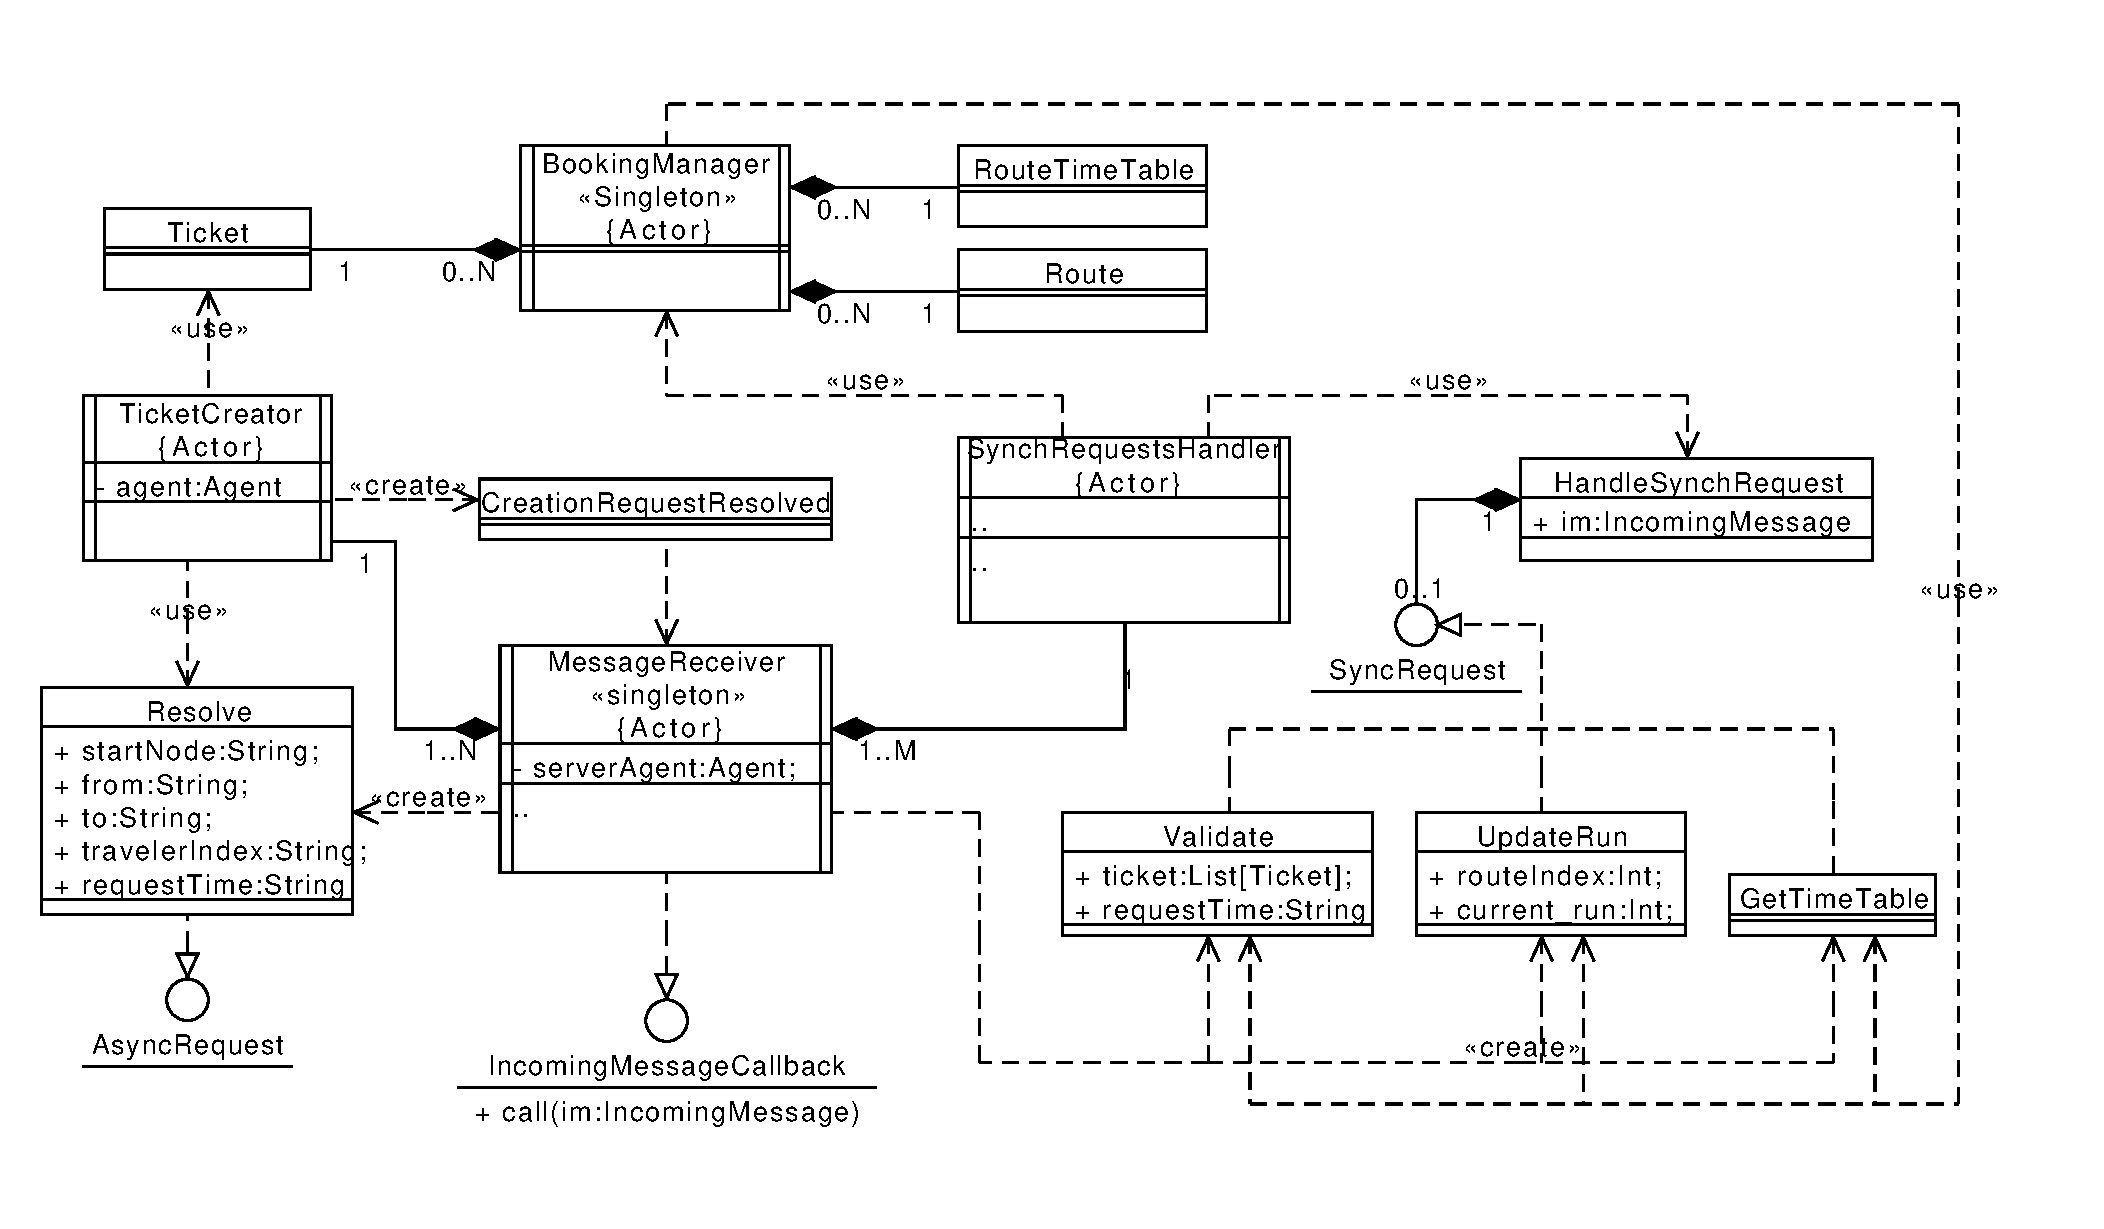
\includegraphics[scale=0.5,trim= 35mm 0mm 0mm 0mm]{imgs/ticket_office_class.pdf}
		\caption{\footnotesize{Diagramma delle classi semplificato che mostra le relazioni principali tra le classi che compongono la Biglietteria Centrale.}}
		\label{img:ticket_office_class_diagram}
	\end{figure}
	
	Il diagramma delle classi in figura \ref{img:ticket_office_class_diagram} presenta l'architettura di massima della componente. La dicitura \ttt{Actor} indica che la classe estende la classe astratta \ttt{scala.actors.Actor}. Di seguito verrà effettuate una breve descrizione delle classi più importanti, e verrà utilizzato il concetto di \ii{Attore} utilizzato dal linguaggio Scala.
	
	\subsection{MessagesReceiver}
	
	La classe Singleton \ttt{MessagesReceiver}, rappresenta un \ii{Attore} il cui compito è ricevere messaggi remoti (implementa infatti l'interfaccia \ttt{IncomingMessageCallback}). Tra i parametri principali mantenuti dall'unico oggetto di tipo \ttt{MessagesReceiver}, vi sono un'istanza di agente messo a disposizione dal middleware \ii{Yami4} per la ricezione dei messaggi remoti, e due array di oggetti, rispettivamente di tipo \ttt{TicketCreator} e \ttt{SynchRequestsHandler}. 
	In base al tipo di richiesta remota ricevuta, l'oggetto \ttt{MessagesReceiver} delega la gestione del messaggio ad uno degli attori nei due array, a seconda se la richiesta è di natura asincrona o sincrona. I tipi di messaggio remoto ricevuti possono essere:
	\begin{itemize}
		\item \ttt{create\_ticket}: richiesta di creazione di un Ticket, che viene delegata ad uno degli attori di tipo \ttt{TicketCreator} mantenuti, inviando ad esso un messaggio di tipo \ttt{Resolve}. Il risultato dell'operazione richiesta viene restituito in maniera asincrona al richiedente.
		\item \ttt{get\_time\_table}: richiesta effettuata da un Nodo di simulazione per ottenere la tabella degli orari. La natura della richiesta è sincrona, e viene quindi delegata ad uno degli attori di tipo \ttt{SynchRequestsHandler}, inviando ad esso un messaggio di tipo \ttt{HandleSynchRequest}.
		
		\item \ttt{update\_run}: richiesta di aggiornamento della corsa corrente, anch'essa di natura sincrona e quindi delegata ad un \ii{Attore} di tipo \ttt{SynchRequestsHandler}, inviando ad esso un messaggio di tipo \ttt{HandleSynchRequest}.
		
		\item \ttt{validate}: richiesta di validazione di un dato Ticket, anch'essa di natura sincrona e quindi delegata ad un \ii{Attore}  di tipo \ttt{SynchRequestsHandler}, inviando ad esso un messaggio di tipo \ttt{HandleSynchRequest}.
		
		\item \ttt{marker}: messaggio effettuato per attuare la procedura di terminazione della Biglietteria Centrale; alla ricezione del primo \ttt{marker}, l'oggetto \ttt{MessagesReceiver} inserisce le successive richieste di creazione di un Ticket in una coda apposita, alla seconda ricezione richiede la terminazione di tutti gli attori attivi mediante l'invio di un messaggio \ttt{Stop}.		
		
	\end{itemize}
	
	\subsection{TicketCreator}
	
	La classe \ttt{TicketCreator} rappresenta un \ii{Attore} incaricato di creare un Biglietto. Esso svolge le seguenti operazioni:
	\begin{itemize}
		\item Ricerca del Nodo (ovvero della Regione) nel quale la stazione di destinazione è contenuta.
		\item Una volta individuato il Nodo, costruzione di un \ii{percorso} attraverso più Nodi per il raggiungimento della destinazione.
		\item Richiesta di creazione di porzioni di Ticket ai Nodi del \ii{percorso}.
		\item Validazione dei Biglietti ottenuti attraverso l'invio di un messaggio all'attore \ttt{BookingManager}.
		\item Unione dei vari Ticket in un unico Biglietto.
		\item Restituzione del Biglietto creato o segnalazione di errore se la procedura non è stata completata.
	\end{itemize}

	\subsection{SynchRequestsHandler}
	
	La classe \ttt{SynchRequestsHandler} rappresenta un \ttt{Attore} incaricato di gestire le richieste sincrone di validazione di un biglietto, di aggiornamento della corsa corrente, e di ottenimento della tabella degli orari. Esso attende fino al completamento dell'operazione assegnata, al termine della quale invia un messaggio di risposta opportuno al richiedente, tramite l'oggetto di tipo \ttt{IncomingMessage} contenuto nel messaggio \ttt{HandleSynchRequest} ricevuto.	
	
	\subsection{BookingManager}
	
	L'\ii{Attore} \ttt{BookingManager} rappresenta una entità \ii{server} a protezione delle tabelle orarie e delle prenotazioni. Esso ha il compito di serializzare gli accessi a queste risorse, in modo tale da evitare modifiche inconsistenti ai dati in esse contenuti.
	Esso gestisce messaggi di tipo \ttt{UpdateRun} per aggiornare l'indice della corsa corrente di un Treno, di tipo \ttt{Validate} per verificare la disponibilità di posti a sedere per la lista di Ticket ricevuta, e di tipo \ttt{GetTimeTable} per l'ottenimento della tabella degli orari.
	
	\section{Server dei Nomi}
	
	Il Server dei Nomi è realizzato mediante un unico oggetto \ii{Attore} \ttt{NameServer}, il quale implementa l'interfaccia \ttt{IncomingMessageCallback}. Esso mantiene un'istanza della classe \ttt{Agent}, per poter ricevere messaggi remoti ad un dato indirizzo, e una tabella per memorizzare le coppie \ttt{<entità,indirizzo>}. I messaggi remoti che esso può ricevere sono:
	\begin{itemize}
		\item \ttt{bind}: Permette al richiedente di registrare una nuova coppia \ttt{<entità,indirizzo>}; se l'identificativo dell'entità è già presente, esso viene sovrascritto.
		\item \ttt{resolve}: Dato un identificativo di entità, restituisce, se presente nella tabella, l'indirizzo al quale quell'entità si trova.
		\item \ttt{list}: Restituisce tutte le coppie \ttt{<entità,indirizzo>} possedute.
		\item \ttt{remove}: Rimuove dalla tabella la voce corrispondente all'identificativo passato.
	\end{itemize}
	
	\section{Controllo Centrale}
	
	L'entità di Controllo Centrale è responsabile della ricezione degli eventi generati dalla Simulazione, della gestione del meccanismo \ttt{Publish/Subscribe}, e della gestione della Terminazione dell'intero sistema.
	Essa è composta dall'oggetto \ttt{ControllerMain}, il quale mantiene una istanza della classe \ttt{Receiver}, utilizzata per la ricezione dei messaggi remoti, dall'oggetto \ii{Attore} \ttt{Controller} che gestisce la pubblicazione di eventi e la Terminazione, e dall'oggetto \ttt{ControllerView}, il quale gestisce una interfaccia grafica per permettere l'interazione dell'utente.
	La classe \ttt{Receiver} contiene un istanza di agente remoto, e riceve i seguenti tipi di messaggio remoto:
	\begin{itemize}
		\item \ttt{event}: Rappresenta un evento, che viene inviato all'oggetto \ttt{Controller} mediante un messaggio di tipo \ttt{Event}.
		\item \ttt{central\_office\_ack}: Rappresenta il messaggio inviato dalla Biglietteria Centrale per comunicare l'avvenuta terminazione delle richieste pendenti; alla ricezione di questo messaggio viene inviato un messaggio \ttt{Continue} all'oggetto \ttt{Controller} per portare a termine la procedura di Terminazione.
		\item \ttt{node\_terminated}: Messaggio inviato da un Nodo per notificare l'avvenuta terminazione. Alla ricezione di tale messaggio, viene inviato un messaggio \ttt{NodeTerminated} all'oggetto \ttt{Controller}.
	\end{itemize}
	L'oggetto \ttt{Controller} gestisce i seguenti messaggi:
	\begin{itemize}
		\item \ttt{Event}, che rappresenta un evento di simulazione, il quale viene pubblicato tramite l'istanza di agente mantenuta.
		\item \ttt{DistributedStop}, inviato da \ttt{ControllerView} a seguito dell'interazione dell'utente con la componente grafica. Alla ricezione viene inviato un messaggio remoto \ttt{marker} alla Biglietteria Centrale.
		\item \ttt{Continue}, alla cui ricezione viene completata la procedura di terminazione, inviando a ciascun Nodo di simulazione una richiesta di terminazione. 
		\item \ttt{NodeTerminated}, che indica la terminazione di uno specifico Nodo. Una volta che tutti i Nodi sono terminati, viene inviato un secondo \ttt{marker} alla Biglietteria Centrale. 
	\end{itemize}
